% !TeX root = ../tesis.tex

Let $\vb{E}^\text{i} = \vb{E}^\text{i}_0 \exp(i\vb{k}^\text{i}\cdot\vb{r})$ be the electric field of an incident monochromatic plane wave with constant amplitude $\vb{E}_0^\text{i}$ \index{Wave!Plane!Monochromatic} traveling through a non-dispersive medium with refractive index $n_\text{m}$, denominated matrix, in the direction $\vb{k}^\text{i} = k_\text{m}\vu{k}^\text{i}$, with $k_\text{m}$ the wave number of the plane wave into the matrix, and let $\vb{E}^\text{sca}$ the electric far field of the scattered field due to a particle with arbitrary shape embedded into the matrix. In general, the scattered electric field propagates in all directions but for a given point $\vb{r} = r\vu{e}_r$ the traveling direction is defined by the vector $\vb{k}^\text{sca} = k_\text{m}\vu{k}^\text{sca} = k_\text{m}\vu{e}_r$.  Due to the linearity of the Maxwell's equations,   the incident and scattered electric fields are related in the far field by a linear relation \cite{tsang_scattering_2000}, that is,
%
% ---------------------------------- eq: ScatAmpMat ----------------------------------
 \begin{equation}
	\vb{E}^\text{sca} =   \frac{\exp(i\vb{k}^\text{sca}\cdot\vb{r})}{r} \mathbb{F}(\vu{k}^\text{sca}, \vu{k}^\text{i}) \vb{E}^\text{i},
 \label{eq:ScatAmpMat}
 \end{equation}
% ---------------------------------- eq: ScatAmpMat ----------------------------------
%
where $\mathbb{F}(\vu{k}^\text{sca}, \vu{k}^\text{i})$ is the scattering  amplitude matrix from direction $\vu{k}^\text{i}$ into $\vu{k}^\text{sca}$\index{Scattering!Amplitude Matrix}. Since only the far field is considered, both the incident and the scattered electric field can be decomposed into two linearly independent components perpendicular to $\vb{k}^\text{i}$ and $\vb{k}^\text{sca}$, respectively, each forming a right-hand orthonormal system. If the particle acting as a scatterer has a symmetric shape, it is convenient to define the orthonormal systems relative to the scattering plane\index{Plane!Scattering}, which is the plane containing $\vb{k}^\text{i}$ and $\vb{k}^\text{sca}$, since the elements of $\mathbb{F}(\vu{k}^\text{sca}, \vu{k}^\text{i})$ simplify when represented in these bases \cite{tsang_scattering_2000}. By defining the directions perpendicular  ($\perp$) and parallel ($\parallel$) to the scattering plane, the incident and scattered electric fields can be written as
%
% ---------------------------------- eq:Ei // eq:Es ------------------------------
 \begin{align}
	\vb{E}^\text{i} & =  \qty(E_\parallel^\text{i}\vu{e}^\text{i}_\parallel + E_\perp^\text{i} \vu{e}_\perp^\text{i}) \exp(i\vb{k}^\text{i}\cdot\vb{r}),
 \label{eq:Ei} \\
	\vb{E}^\text{sca} & = \qty(E_\parallel^\text{sca}\vu{e}^\text{sca}_\parallel + E_\perp^\text{sca} \vu{e}_\perp^\text{sca}) \frac{\exp(i\vb{k}^\text{sca}\cdot\vb{r})}{r},
 \label{eq:Es}
 \end{align}
% ---------------------------------- eq:Ei // eq:Es ------------------------------
%
where the harmonic time dependence  $\exp(-i\omega t)$ has been suppressed, and where it has been assumed that the scattered field is described by a spherical wave; the superindex ``$\text{i}$'' (``$\text{sca}$'') denotes the orthonormal system defined by the incident plane wave (scattered fields).  Since $\{\vu{e}_\perp^\text{i}, \vu{e}_\parallel^\text{i},\vu{k}^\text{i} \}$ and $\{\vu{e}_\perp^\text{sca}, \vu{e}_\parallel^\text{sca},\vu{k}^\text{sca} \}$ are right-hand orthonormal systems, they are related by
%
% ---------------------------------- eq:eParaPerpPerp ------------------------------
 \begin{align}
	\vu{e}_\perp^\text{i} = \vu{e}_\perp^\text{sca}  & =  \vu{k}^\text{sca} \times \vu{k}^\text{i},
		\qquad\qquad
	\vu{e}^\text{i}_\parallel = \vu{k}^\text{i}\times \vu{e}^\text{i}_\perp,
		\qquad\qquad
	\vu{e}^\text{sca}_\parallel = \vu{k}^\text{sca} \times \vu{e}_\perp^\text{sca}.
 \label{eq:eParaPerp}
 \end{align}
% ---------------------------------- eq:eParaPerpPerp ------------------------------
%

As the Eqs. \eqref{eq:eParaPerp} suggest, the unit vector bases of the orthonormal systems relative to the scattering plane depend on the scattering direction. For example, if the incident plane wave travels along the $z$ axis, then $\vu{k}^\text{i} = \vu{e}_z$ and $\vu{k}^\text{sca} = \vu{e}_r$. Thus, according to Eqs. \eqref{eq:eParaPerp}, the unit vector bases of the systems relative to the scatterig plane are   $\vu{e}_\parallel^\text{i} = \cos\varphi \vu{e}_x +\sin\varphi \vu{e}_y$, $\vu{e}_\parallel^\text{sca} = \vu{e}_\theta$ and $\vu{e}_\perp^\text{i} = \vu{e}_\perp^\text{sca}  = - \vu{e}_\varphi$, with $\theta$ the polar angle and $\varphi$ azimuthal angle. In Fig. \ref{fig:ScatPlane} the unit vector systems (purple) based on the  scattering plane  (green) defined by the vectors $\vu{k}^\text{i}=\vu{e}_z$ and $\vu{k}^\text{sca} = \vu{e}_r$ are shown, along with the Cartesian (blue) and spherical (black) unit vector bases.

\begin{figure}[h!]\centering
	\tdplotsetmaincoords{60}{110}
	\pgfmathsetmacro{\rvec}{1. 3}
	\pgfmathsetmacro{\thetavec}{30}
	\pgfmathsetmacro{\varphivec}{60}
\begin{tikzpicture}[scale=3.5,tdplot_main_coords]
%draw the NP
%	\draw[tdplot_screen_coords,ball color=yellow, opacity = 1] (0,0,0) circle (.05);
%	\draw[tdplot_screen_coords, color=yellow, opacity = 1] (0,0,0) circle (.05);

\pgfmathsetseed{3}
\draw[tdplot_screen_coords, ball color=yellow, opacity = 1,scale =.075]
	 plot [smooth cycle, samples=8,domain={1:8}]
     (\x*360/8+5*rnd:0.5cm+1cm*rnd) node at (0,0) {};
\pgfmathsetseed{3}
\draw[tdplot_screen_coords, color=yellow, opacity = 1,scale =.075]
	 plot [smooth cycle, samples=8,domain={1:8}]
     (\x*360/8+5*rnd:0.5cm+1cm*rnd) node at (0,0) {};


%set up some coordinates
	\coordinate (O) at (0,0,0);

%determine a coordinate (P) using (r,\theta,\varphi) coordinates.   This command
%also determines (Pxy), (Pxz), and (Pyz): the xy-, xz-, and yz-projections
%of the point (P).
%syntax: \tdplotsetcoord{Coordinate name without parentheses}{r}{\theta}{\varphi}
	\tdplotsetcoord{P}{\rvec}{\thetavec}{\varphivec}

%draw figure contents
%--------------------
%draw the main coordinate system axes
	\draw[thick,- latex] (0,0,0) -- (1. 5,0,0) node[anchor=north east]{$x$};
	\draw[thick,- latex] (0,0,0) -- (0,1. 5,0) node[anchor=north west]{$y$};
	\draw[thick,- latex] (0,0,0) -- (0,0,1. 5) node[anchor=south]{$z$};

%draw the main cartesian vector system
	\draw[thick,- latex, blue] (0,0,0) -- (1,0,0) node[anchor= south east]{$\vu{e}_x$};
	\draw[thick,- latex, blue] (0,0,0) -- (0,1,0) node[anchor=north west]{$\vu{e}_y$};
	\draw[thick,- latex, blue] (0,0,0) -- (0,0,1) node[anchor= east]{$\vu{e}_z$};

%draw a vector from origin to point (P)
	\draw[thick,color=green, - latex] (O) -- (P);
	\node at (1,. 5,1. 1) {\color{green} $\vb{r}$};

%draw projection on xy plane, and a connecting line
	\draw[dashed, color=green] (O) -- (Pxy);
	\draw[dashed, color=green] (P) -- (Pxy);
	\fill[green, opacity = .3] (O) --(Pxy)-- (P)--(O);
	\draw[- latex, tdplot_screen_coords,green](.42,.2)--(.8,.2);
	\node[tdplot_screen_coords] at (1.2,.2) {\color{green}\small Scattering plane};


%draw the angle \varphi, and label it
	%syntax: \tdplotdrawarc[coordinate frame, draw options]{center point}{r}{angle}{label options}{label}
	\tdplotdrawarc[- latex]{(O)}{0. 5}{0}{\varphivec}{anchor=south}{$\varphi$}


%set the rotated coordinate system so the x'-y' plane lies within the
	%"theta plane" of the main coordinate system
	%syntax: \tdplotsetthetaplanecoords{\varphi}
	\tdplotsetthetaplanecoords{\varphivec}

%draw theta arc and label, using rotated coordinate system
	\tdplotdrawarc[tdplot_rotated_coords, - latex]{(0,0,0)}{0. 45}{0}{\thetavec}{anchor=north}{$\theta$}

%draw some dashed arcs, demonstrating direct arc drawing
	\draw[dashed,tdplot_rotated_coords] (\rvec,0,0) arc (0:90:\rvec);
	\draw[dashed] (\rvec,0,0) arc (0:90:\rvec);

%set the rotated coordinate definition within display using a translation
%coordinate and Euler angles in the "z(\alpha)y(\beta)z(\gamma)" euler rotation convention
%syntax: \tdplotsetrotatedcoords{\alpha}{\beta}{\gamma}
	\tdplotsetrotatedcoords{\varphivec}{\thetavec}{0}

%translate the rotated coordinate system
%syntax: \tdplotsetrotatedcoordsorigin{point}
	\tdplotsetrotatedcoordsorigin{(P)}

%use the tdplot_rotated_coords style to work in the rotated, translated coordinate frame
	\draw[thick,tdplot_rotated_coords,- latex, purple] (0,0,0) -- (. 3,0,0) node[anchor=north west]{{\color{black}$\vu{e}_\theta,$}$\vu{e}_{\parallel}^\text{sca}$};
	\draw[thick,tdplot_rotated_coords,- latex,black] (0,0,0) -- (0,. 3,0) node[anchor=west]{$\vu{e}_\varphi$};
	\draw[thick,tdplot_rotated_coords,- latex,purple] (0,0,0) -- (0,-. 3,0) node[anchor= north west]{$\vu{e}_{\perp}^\text{sca}$};
	\draw[thick,tdplot_rotated_coords,- latex] (0,0,0) -- (0,0,. 3) node[anchor=south]{$\vu{k}^\text{sca}, \vu{e}_r$ };



%set the rotated coordinate definition within display using a translation
%coordinate and Euler angles in the "z(\alpha)y(\beta)z(\gamma)" euler rotation convention
%syntax: \tdplotsetrotatedcoords{\alpha}{\beta}{\gamma}
	\tdplotsetrotatedcoords{\varphivec}{0}{0}

%translate the rotated coordinate system
%syntax: \tdplotsetrotatedcoordsorigin{point}
	\tdplotsetrotatedcoordsorigin{(Pxy)}

	\draw[thick,tdplot_rotated_coords,- latex, purple] (0,0,0) -- (. 3,0,0) node[anchor= west]{$\vu{e}_{\parallel}^\text{i}$};
	\draw[thick,tdplot_rotated_coords,- latex, blue] (0,0,0) -- (0,0,. 3) node[anchor= west]{$\vu{e}_z$};
	\draw[thick,tdplot_rotated_coords,- latex, purple] (0,0,0) -- (0,-. 3,0) node[anchor= north west]{$\vu{e}_{\perp}^\text{i}$};



% Plane Wave
	\foreach \i in {-7,...,-2}{
		\draw[thick,tdplot_screen_coords,red, - latex] (\i/10,0,0)--(\i/10,1,0);}
	\node[tdplot_screen_coords] at (-4.5/10,1.1,0){\color{red}$\vb{k}_i$};
	\node[tdplot_screen_coords] at (-4.5/10,-.15,0){\begin{minipage}{2.cm}\centering\small \color{red}Incident plane wave\end{minipage}};
\end{tikzpicture}
%
\caption[Scattering plane unit vector systems]{The scattering plane (green) is defined by the vectors $\vu{k}^\text{i}$, direction of the incident plane wave (red), and $\vu{k}^\text{sca}$, direction of the scattered field in a given point $\vec{r}$. If the direction of the incident plane wave is chose to be $\vu{e}_z$, the parallel and perpendicular components of the incident field relative to the scattering plane are $\vu{e}_\parallel^\text{i} = \cos\varphi\vu{e}_x +\sin\varphi\vu{e}_y$ and  $\vu{e}_\perp^\text{i} = -\vu{e}_\varphi$, while the components of the scattering field relative to the scattering plane are $\vu{e}_\parallel^\text{sca} = \vu{e}_\theta$, $\vu{e}_\perp^\text{sca} = - \vu{e}_\varphi$. The cartesian unit vector basis is shown in blue, the spherical unit vector basis in black, while the basis of the orthonormal systems relative to the scattering plane are shown in purple. }
\label{fig:ScatPlane}
	\end{figure}

After a incident plane wave interacts with a particle with a possible complex refractive index $n_p(\omega)$, the total electric field outside the particle is given by the sum of the incident and the scattered fields. Therefore, the time averaged Poynting vector $\ev{\vb{S}}_t$, denoting the power flow per unit area, of the total field is given by
%
% ---------------------------------------------------------
 \begin{align}
	\ev{\vb{S}}_t
		= \underbrace{\frac12 \Re \qty(\vb{E}^\text{i}\times\vb{H}^\text{i*})}_{\text{\normalsize $\ev{\vb{S}^\text{i}}_t $}} +
		\underbrace{\frac12 \Re \qty(\vb{E}^\text{sca}\times\vb{H}^\text{sca*})}_{\text{\normalsize $\ev{\vb{S}^\text{sca}}_t $}}+
		\underbrace{	\frac12 \Re\qty(\vb{E}^\text{i}\times\vb{H}^\text{sca*} + \vb{E}^\text{sca}\times\vb{H}^\text{i*})}_{\text{\normalsize$\ev{\vb{S}^\text{ext}}_t$}},
 \label{eq:Stot}
 \end{align}
% ---------------------------------------------------------
%
where $(*)$ denotes the complex conjugate operation and where the total Poynting vector is separated into the contribution from the incident field $\ev{\vb{S}^\text{i}}_t$, from the scattered field $\ev{\vb{S}^\text{sca}}_t$ and from their cross product denoted by $\ev{\vb{S}^\text{ext}}_t$. By means of the Faraday-Lenz\index{Faraday-Lenz!Law}\index{Law!Faraday-Lenz}\index{Maxwell!Equations} Law and Eq. \eqref{eq:ScatAmpMat}, the  contribution to the Poynting vector from the incident and the scattered fields can be rewritten as\index{Poynting vector}
%
% ------------------ Si
 \begin{equation}
	\ev{\vb{S}^\text{i}}_t = \frac{\norm{\vb{E}_0^\text{i}}^2}{2 Z_\text{m}}\vu{k}^\text{i},
		\qquad\text{and}\qquad
	\ev{\vb{S}^\text{sca}}_t = \frac{\norm{\vb{E}^\text{sca}}^2}{2 Z_\text{m}}\vu{k}^\text{sca}
						=  \frac{\norm{\mathbb{F}(\vu{k}^\text{sca},\vu{k}^\text{i})\vb{E}^\text{i}}^2}{2 Z_\text{m}r^2}\vu{k}^\text{sca},
 \label{eq:AvePoyntingISca}
 \end{equation}
% ------------------- Si
%
with $Z_\text{m} = \sqrt{\mu_\text{m}/\varepsilon_\text{m}}$, the impedance of the non-dispersive matrix, while the crossed contribution is given by
%
% ------------------ Si
 \begin{align}
 \ev{\vb{S}^\text{ext}}_t = &\Re\left\{
								\frac{\exp[-i(\vb{k}^\text{sca}-\vb{k}^\text{i})\cdot\vb{r}]}{2 Z_\text{m}r^2}
								\qty[\vu{k}^\text{sca}\qty(\vb{E}_0^\text{i}\cdot \mathbb{F}^*\vb{E}^\text{i*})
									-\mathbb{F}^*\vb{E}^\text{i*}	\qty(\vb{E}^\text{i}_0\cdot\vu{k}^\text{sca})]
							 \right.\notag	\\
							&\hspace{2em}\left.
								+\frac{\exp[i(\vb{k}^\text{sca}-\vb{k}^\text{i})\cdot\vb{r}]}{2 Z_\text{m}r^2}
								\qty[\vu{k}^\text{i}\qty(\mathbb{F}\vb{E}^\text{i}\cdot\vb{E}^\text{i*}_0)
									-\vb{E}^\text{i*}_0 \qty(\mathbb{F}\vb{E}^\text{i}\cdot\vu{k}^\text{i})]	\right\},
 \label{eq:AvePoyntingExt}
 \end{align}
% ------------------- Si
%
where the scattering amplitude matrix is evaluated as $\mathbb{F}(\vu{k}^\text{sca},\vu{k}^\text{i})$.

The power scattered by the particle can be calculated by integrating $\ev{\vb{S}^\text{sca}}_t$ in a closed surface surrounding the particle; if the scattered power is normalized by the irradiance\index{Plane Wave!Irradiance}\index{Irradiance} of the incident field $\norm{\ev{\vb{S}^\text{i}}_t}$, it is obtained a quantity with units of area known as the scattering cross section $C_\text{sca}$, given by
%
% ------------------ Si
 \begin{tcolorbox}[title = Scattering Cross Section,	ams align, breakable]
	C_\text{sca} = \frac{2Z_\text{m}}{\norm{\vb{E}_0}^2}\oint\ev{\vb{S}^\text{sca}}\cdot\dd{\vb{a}}
				= \oint\frac{\norm{\mathbb{F}(\vu{k}^\text{sca},\vu{k}^\text{i})\vb{E}^\text{i}}^2}
									{\norm{\vb{E}^\text{i}_0}^2}\dd{\Omega},
 \label{eq:Csca}
 \end{tcolorbox}
% ------------------- Si
%
\noindent where $\dd{\Omega}$ is the solid angle differential.
In a similar manner, an absorption cross section $C_\text{abs}$ can be defined as well. On the one side, the absorption cross section is given by the integral on a closed surface of $-\ev{\vb{S}}_t$  [Eq. \eqref{eq:Stot}] divided by the irradiance of the incident field, where the minus sign is chosen so that $C_\text{abs}>0$ if the particle absorbs energy  \cite{bohren_absorption_1983}. On the other side, if an Ohmic material for the particle\index{Ohm!Law} with a conductivity $\sigma(\omega) = i\omega n_p^2(\omega)$ \cite{jackson_classical_1999} is assumed, through Joule's Heating Law \cite{tsang_scattering_2000}\index{Joule!Heating Law} the absorption cross section can be computed as
%
% ------------------ Si
 \begin{tcolorbox}[title = Ohmic Particle - Absorption Cross Section,	ams align, breakable]
 	C_\text{abs} =	 \frac12\int \frac{\Re(\vb{j}\cdot \vb{E}^\text{int*})}
 									{\norm{\vb{E}_0^\text{i}}^2/2Z_\text{m}}\dd{V}
				= \int\omega Z_\text{m}\Im(n_p^2) \frac{\norm{\vb{E}^\text{int}}^2}{\norm{\vb{E}^\text{i}_0}^2} \dd{V},
 \label{eq:Cabs}
 \end{tcolorbox}%
% ------------------- Si
%
\noindent where integration is performed inside the particle, and $\vb{j}$  and $\vb{E}^\text{int}$, are the volumetric electric current density and the total electric field in this region. Both the  scattering and the absorption cross sections are quantities related to the optical signature of a particle \cite{pellarin_forward_2019}, and their relation can be made explicit by performing the surface integral representation of $C_\text{abs}$ and defining $C_\text{ext}$, that is,
%
% -----------------------------
\begin{align}
C_\text{abs} = & - \frac{2Z_\text{m}}{\norm{\vb{E}^\text{i}_0}^2}\int\Big(\ev{\vb{S}^\text{i}}_t + \ev{\vb{S}^\text{sca}}_t + \ev{\vb{S}^\text{ext}}_t\Big)\cdot\dd{\vb{a}}
					\notag \\
			=  & - C_\text{sca} - \frac{2Z_\text{m}}{\norm{\vb{E}_0^\text{i}}^2}\int   \ev{\vb{S}^\text{ext}}_t\cdot \vu{e}_r\dd{\Omega}
					\notag \\
			= & -C_\text{sca} + C_\text{ext},
\label{eq:CabsScaInt}
\end{align}
% ------------------------------
%
where the contribution of $\ev{\vb{S}^\text{i}}_t$ to the integral is zero since a non-dispersive matrix was assumed. From Eq.\eqref{eq:CabsScaInt} it can be seen that $C_\text{ext}$ takes into account both mechanisms for energy loses (scattering and absorption), thus it is called the extinction cross section\index{Extinction!Cross Section}. To solve the integral in Eq. \eqref{eq:CabsScaInt} let us define $\theta$ as the angle between $\vu{k}^\text{sca}$ and $\vu{k}^\text{i}$ as the polar angle  and  $\varphi$ as the azimuthal angle as shown in Fig \ref{fig:ScatPlane}. With this election of coordinates,  the extinction cross section can be computed as
%
% -----------------------------
\begin{align}
C_\text{ext} = - &\Re \left\{
			 \frac{\exp(-ik_mr) }{\norm{\vb{E}_0^\text{i}}^2}
			 					\oint \exp(ik_mr\cos\theta)(1)\qty(\vb{E}^\text{i}\cdot \mathbb{F}^*\vb{E}^\text{i*})  \dd{\Omega} \right.	\notag\\
			&\hspace*{1.5em}+\frac{\exp(ik_mr) }{\norm{\vb{E}_0^\text{i}}^2}
								\oint \exp(-ik_mr\cos\theta)\cos\theta \qty(\vb{E}^\text{i*}\cdot \mathbb{F}\vb{E}^\text{i})     \dd{\Omega}
\label{eq:CextFull}\\
			&\hspace*{1.5em}+\left.\frac{\exp(ik_mr) }{\norm{\vb{E}^\text{i}_0}^2}
								\oint \exp(-ik_mr\cos\theta)\sin\theta(E_{0,x}^\text{i}\cos\varphi+E_{0,y}^\text{i}\sin\varphi)
									\qty(\mathbb{F}\vb{E}^\text{i}\cdot\vb{k}^\text{i})    \dd{\Omega}  \right\} \notag
\end{align}
% ------------------------------
%
where the relations $\vu{k}^\text{sca}\cdot\vu{e}_r = 1$, $\vu{k}^\text{i}\cdot\vu{e}_r = \cos\theta$ and  $\vb{E}^\text{sca}\cdot\vu{e}_r = 0$ were employed. The integrals in Eq. \eqref{eq:CextFull} can be solved by a two fold integration by parts on the polar angle $\theta$ and by depreciating the terms proportional to $r^{-2}$. This process leads to a zero contribution from the integrand proportional to $\sin\theta$  of Eq. \eqref{eq:CextFull}, and after arranging the other terms in their real and imaginary parts, it follows that $C_\text{ext}$ depends only in the forward direction  $\vu{k}^\text{sac} = \vu{k}^\text{i}$ ($\theta =0$). This result is known as the Optical Theorem\index{Optical!Theorem} and whose mathematical expression is given by \cite{tsang_scattering_2000,pellarin_forward_2019,newton_optical_1976}
%
% -----------------------------
\begin{tcolorbox}[title = Optical Theorem - Extinction Cross Section,	ams align, breakable]
		C_\text{ext} = C_\text{abs} + C_\text{sca}
					=  \frac{4\pi}{k_m \norm{\vb{E}_0^\text{i}}^2}&\Im\qty[ \vb{E}_0^\text{i}\cdot \mathbb{F}^*(\vu{k}^\text{i},\vu{k}^\text{i}) \vb{E}^\text{i*} ].
\label{eq:Cext}
\end{tcolorbox}
% ------------------------------
%
\noindent From Eqs. \eqref{eq:Stot} and  \eqref{eq:Cext} it can be seen that the extinction of light, the combined result of scattering and absorption as energy loss mechanisms, is also a manifistation of the interference beteen the incident and the scattered fields and that the over all effect of the light extinction can be fully understood by analizing the  amplitude of the scattering field in the forward direction.  It is woth noting that Eq. \eqref{eq:Cext} is an exact relation but its usefullness is bond to the correct evaluation of the scattereing amplitude matrix $\mathbb{F}$ \cite{tsang_scattering_2000}. Thus, in the following sections a scattering problem with spherical symmery will be assumed, so that the exact solution to the scatterng amplitude matrix can be developed; this solution is known as Mie Theory.

 %The Optical Theorem is a general result no only applicable to  for general scattering phenomena, both quantum and classical  \cite{bohren_absorption_1983,newton_optical_1976}, its derivation rely in the incident field being a plane wave [see Eq. \eqref{eq:CextFull}] and more precisely, in the lack of longitudinal components of the incident field \cite{krasavin_generalization_2018,born_max_principle_1999}.







\clearpage

\begin{figure}
\def\svgwidth{\textwidth} \small
%\input{1-Theory-Figs/redShift.pdf_tex}%
\includeinkscape{1-Theory-Figs/redShift}%
\vspace*{-23.75em}
\hspace*{-4.5em}
\begin{subfigure}{.24\textwidth}\caption{ }\label{1}\end{subfigure}
\begin{subfigure}{.24\textwidth}\caption{ }\label{2}\end{subfigure}
\begin{subfigure}{.235\textwidth}\caption{ }\label{3}\end{subfigure}
\begin{subfigure}{.24\textwidth}\caption{ }\label{4}\end{subfigure}
\vspace*{22em}
\caption{   }
\end{figure}

\begin{figure}
%\input{1-Theory-Figs/redShift.pdf_tex}%
\includegraphics[width=\textwidth]{1-Theory-Figs/redShift_proof.pdf}
\vspace*{-23.75em}
\hspace*{-4.5em}
\begin{subfigure}{.24\textwidth}\caption{ }\label{1}\end{subfigure}
\begin{subfigure}{.24\textwidth}\caption{ }\label{2}\end{subfigure}
\begin{subfigure}{.235\textwidth}\caption{ }\label{3}\end{subfigure}
\begin{subfigure}{.24\textwidth}\caption{ }\label{4}\end{subfigure}
\vspace*{22em}
\caption{   }
\end{figure}


%


%
\begin{figure}[h!]\centering
	\begin{subfigure}{.05\textwidth}\caption{}\label{•}label{sfig:secondary1}\vspace*{5.5cm}\end{subfigure}
	\hspace*{-2.em}
	\begin{subfigure}{.48\textwidth} 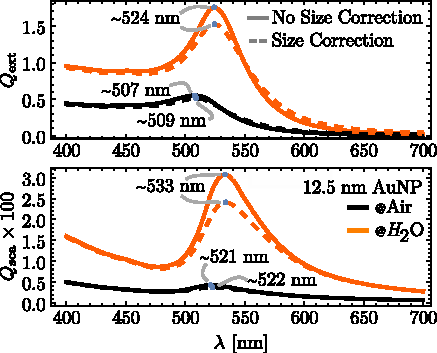
\includegraphics[scale = 1.02]{1-Theory/figs/QextQsca_12-5.pdf}\end{subfigure}
	\hspace*{-.5em}\begin{subfigure}{.05\textwidth}\vspace{-5.5cm}\caption{}\label{sfig:secondaty2}	\end{subfigure}
	\hspace*{-2.em}
	\begin{subfigure}{.48\textwidth} 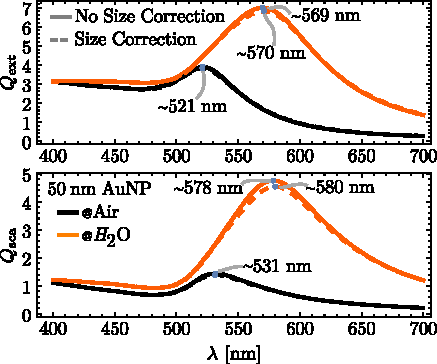
\includegraphics[scale = 1.02]{1-Theory/figs/QextQsca_50.pdf}\end{subfigure}%
\vspace*{-.5em}
\caption[Example of Figure title]{The explanation of your figures. \blindtext}	\label{fig:Main}
\end{figure}

\begin{figure}[h!]\centering
	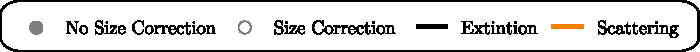
\includegraphics[scale=1]{1-Theory/figs/legend.pdf}\\[.5em]
%
	\hspace*{2em}\begin{subfigure}{.05\textwidth}\caption{}\label{sfig:secondary1}\vspace*{6.35cm}\end{subfigure}
	\hspace*{-3.50em}
	\begin{subfigure}{.24\textwidth} 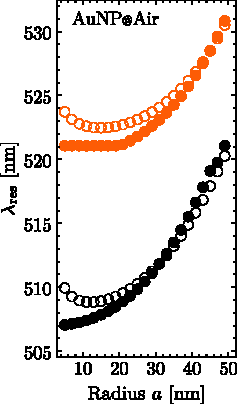
\includegraphics[scale = 1]{1-Theory/figs/redShift_rad1.pdf}\end{subfigure}
%
	\hspace*{.25em}\begin{subfigure}{.05\textwidth}\vspace{-6.35cm}\caption{}\label{sfig:secondaty2}	\end{subfigure}
	\hspace*{-2.5em}
	\begin{subfigure}{.24\textwidth} 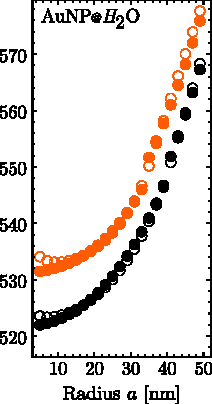
\includegraphics[scale = 1]{1-Theory/figs/redShift_rad2.pdf}\end{subfigure}%
%
	\hspace*{-.5em}\begin{subfigure}{.05\textwidth}\vspace{-6.35cm}\caption{}\label{sfig:secondaty2}	\end{subfigure}
	\hspace*{-2.45em}
	\begin{subfigure}{.24\textwidth} 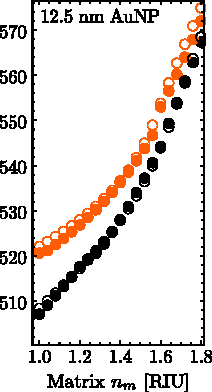
\includegraphics[scale = 1.02]{1-Theory/figs/redShift_mat1.pdf}\end{subfigure}%
%
	\hspace*{-.45em}\begin{subfigure}{.05\textwidth}\vspace{-6.35cm}\caption{}\label{sfig:secondaty2}	\end{subfigure}
	\hspace*{-2.45em}
	\begin{subfigure}{.24\textwidth} 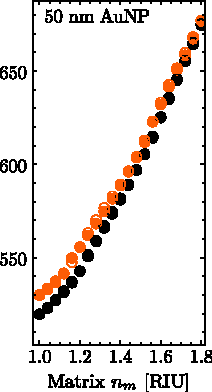
\includegraphics[scale = 1.02]{1-Theory/figs/redShift_mat2.pdf}\end{subfigure}%
\vspace*{-.5em}
\caption[Example of Figure title]{The explanation of your figures. \blindtext}
\label{fig:Main}
\end{figure}
\clearpage
